% !TEX root = ../2021_microservices_wileytemplate.tex

\section{Results}\label{sec:results}

In this section, we present the results from our systematic literature review. First, we show a general overview of the collected paper's characteristics (Section~\ref{sec:results-general}). Then, we present our results to answer our first research question related to challenges (Section~\ref{sec:results-rq1}). Finally, we describe our findings to answer our second question on the topic of technologies (Section~\ref{sec:results-rq2}).

\subsection{General Analysis}\label{sec:results-general}

Figure~\ref{fig:collected-papers-slr} shows an overview of the collected literature references we used in our systematic literature review. In our study, we have a total of 81 references, of which 60 are from scientific sources and 21 come from grey literature. 

\begin{figure*}[h]
    \centering
    \begin{subfigure}[b]{0.40\textwidth}
        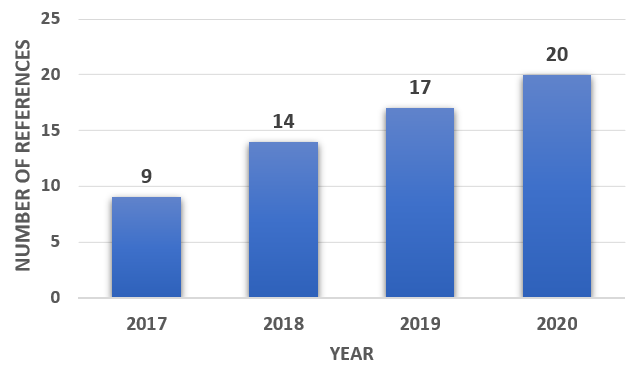
\includegraphics[width=\textwidth]{images/publicationtypes_1.png}
        \caption{Scientific references per year}
        \label{fig:papers-academic-year}
    \end{subfigure}
~
    \begin{subfigure}[b]{0.25\textwidth}
        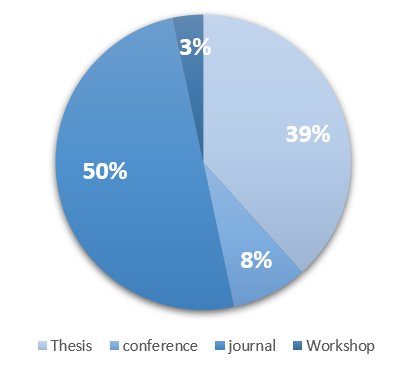
\includegraphics[height=0.2\textheight]{images/publicationtypes_3.png}
        \caption{Types of the scientific references}
        \label{fig:papers-academic-type}
    \end{subfigure}

    \begin{subfigure}[b]{0.40\textwidth}
        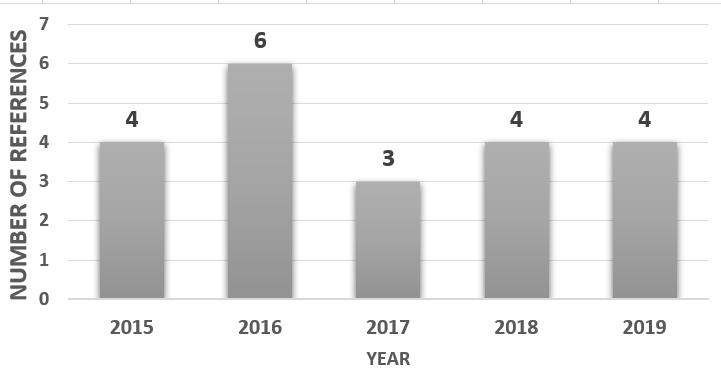
\includegraphics[width=\textwidth]{images/greytype_1.png}
        \caption{Grey references per year}
        \label{fig:papers-grey-year}
    \end{subfigure}
~
    \begin{subfigure}[b]{0.25\textwidth}
        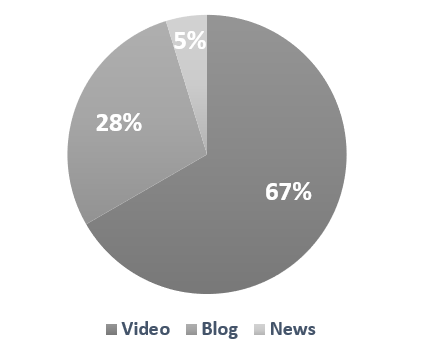
\includegraphics[height=0.2\textheight]{images/greytype_2.png}
        \caption{Types of the grey references}
        \label{fig:papers-grey-type}
    \end{subfigure}

    \caption{collected references Used in the systematic literature Review}\label{fig:collected-papers-slr}

\end{figure*}


We can see the number of scientific references we deemed relevant for our study to grow each year after 2017 (Figure~\ref{fig:papers-academic-year}). Even though we reject papers from before 2017 from our study, we did not design our remaining selection criteria to favor more current papers. Therefore, the rise in the number of references per year is probably just a coincidence. 
%In Figure~\ref{fig:selected-papers-slr-1} We can see the number of papers published after 2017 and the number is growing more every year. In Figure~\ref{fig:selected-papers-slr-2} We can see here the types of publications collected during the SLR \henrique{These are questionable remarks. Since you selected these papers, you cannot claim a generalized trend or a raise.}\keerthana{fixed it}
%
On the other hand, most of the grey literature we used in this study is from 2016 (Figure~\ref{fig:papers-grey-year}). The reason is that the goto conference was our initial starting point to collected grey references. Particularly in 2016, many speakers were discussing microservices in the goto conference.

When we look at the types of literature, we have different classifications for scientific (Figure~\ref{fig:papers-academic-type}) and grey (Figure~\ref{fig:papers-grey-type}). Since all scientific references were papers, we classified them by their publication type (e.g., journal paper, conference paper, thesis). For grey, we classified the references by their media type and publishing format (e.g., video, blog). 
%
%Figure~\ref{fig:selected-papers-grey-1} shows the types of grey literature collected year-wise. There was a total of 21 grey literature which includes blogs, Youtube videos, and News. We could see that there was a lot of grey literature initially published and this serves as a key for practitioners or academia to learn from it and start making more grey literature.
%
From the selected references, we could see there is a good variety of publications. %This may indicate that microservices are discussed in many fields for both the industrial and academia.


\subsection{RQ\#1: What are the main challenges when adopting microservices?}\label{sec:results-rq1}

\begin{figure*}[t]
	\centering
	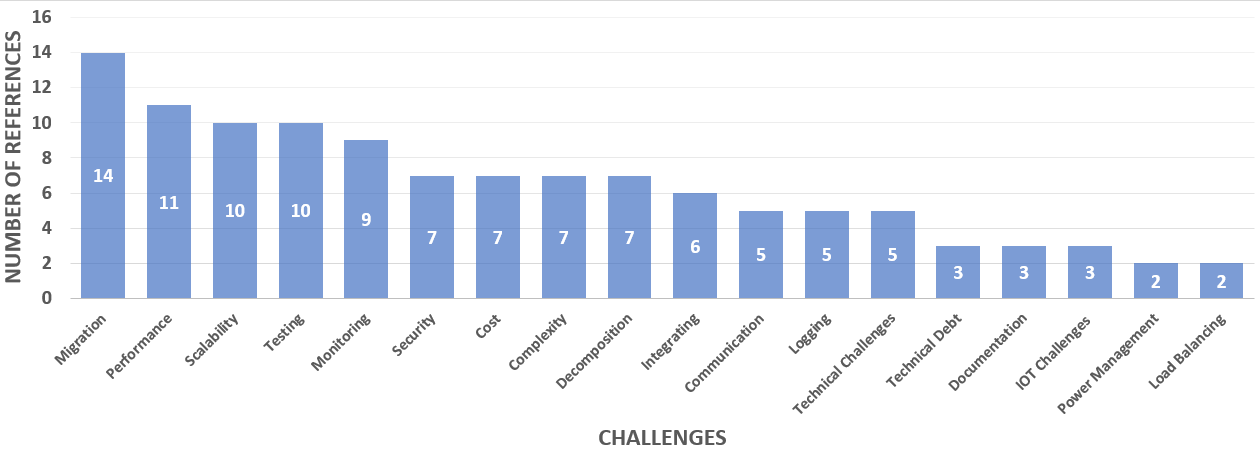
\includegraphics[width=0.9\linewidth]{images/Challenges_updated.png}
	\caption{Challenges in adopting microservices }
	\label{fig:challenges}
\end{figure*}	

In this section, we answer our first research question by analyzing the collected data.
To answer RQ\#1, we examined the spreadsheets created in the data synthesis phase from our 81 references.

Figure~\ref{fig:challenges} shows the challenges in adopting microservices that we discovered in our systematic literature review. It also shows how many distinct references in our selection discuss such challenges. 
According to our classification, we identified \challengecount challenges.
The challenges mentioned on the most number of references are migration and performance, followed by scalability and testing. In our collected data, those are the major challenges of adopting microservices.


\subsubsection{Migration}%#1
When migrating an application the {codebase update~\footnote{Before undertaking any major structural changes, the codebase would have to be updated and unified to make any further changes easier. The technical problems of the outdated codebase, the difficulty of adding new features, and the inferior performance of parts of the application would be targeted}} are difficult tasks as observed from the publication by Tuuli and Wang~\cite{Tuuli2020, wang2020}. 

Database migration is the main problem and risks if the application has a database, and especially its location inside the application docker container. To ensure the stability and maintainability of the application database, it would have to be migrated from its current location to a better alternative ~\cite{Tuuli2020}.

\par Hosting service migration is seen as the main problem in focus during this step were the uneven server load, as well as the difficulty of applying updates to the application~\cite{Tuuli2020}. Many organizations are planning and migrating their on-premise software to the cloud, starting with the Infrastructure as a service (IaaS) and Software as a service (SaaS) models. Nonetheless, they are facing some challenges and difficulties, mainly in the Platform as a service (PaaS) model, related to the complexity in integrating the legacy and internal systems~\cite{rosa2018}. It requires a different way of thinking compared to the traditional way of software architectures, often leading to the migrations and creations of these architectures being long and costly processes~\cite{leo2019}.
\par System application migration is becoming an emerging issue with different challenges. Migration of the system to microservice optimizes decentralization, replaceability, and autonomy of software architectures. Although researchers are not convinced of any specific definition of microservice, its modeling techniques, and its properties, it is aware of system migration to microservices~\cite{ghayyur2018}.
\par Migration of the resulting application towards the new intended state is still a (partially) manual and labor-intensive step~\cite{overeem2018}. If on the one hand microservices can help in achieving a good level of flexibility (e.g., by promoting low services coupling, higher maintainability), on the other hand adopting a microservice-based architecture may bring higher complexity~\cite{Difrancesco2017}. The microservice architectural style has become an essential element for the development of applications deployed on the cloud and for those adopting the devops practices. Nevertheless, while microservices can be used to develop new applications, there are monolithic ones, that are not well adapted neither to the cloud nor to devops. Migrating these applications towards microservices appears as a solution to adapt them to both. 


\par Companies have been widely investing in modernizing the software architecture and development processes of their products. By migrating away from software monoliths towards the emerging microservice architecture style, an agile and robust software system with a compatible development process can be accomplished. Despite this, modernization can be highly challenging from a practical point of view. Available software solutions, which aim at supporting the restructuring of software monoliths into microservices, often do not satisfy the arising demands of the developers. While these products offer diverse static analysis functionalities, dynamic analysis aspects are mostly missing. Yet, especially a dynamic analysis can provide invaluable information about overlooked characteristics of the software system~\cite{Lenga2019}.

\par Serious efforts have been undertaken to move from monolithic architectures to microservice architectures. The common problem in these efforts is to identify from monolithic applications the candidates of microservices which includes the programs or data that can be turned into cohesive, standalone services; this is a tiresome manual effort that requires analyzing many dimensions of software architecture views and often heavily relies on the experience and expertise of the expert performing the extraction~\cite{Kamimura2018}\cite{selmadji2020}.

\subsubsection{Performance}%#2

Goldsmith~\cite{Kevin2015} talks about challenges related to monitoring, latency, and problems with completely autonomous teams. The distributed aspect of a microservice system is a significant challenges~\cite{Matt2016}. Its distributed nature impacts the performance of the system. Calls to a single service might trigger a cascade of additional calls to other services distributed across a network, each adding its latency. The increase in resource usage may cause a microservices-based application to execute slower~\cite{Etsy, Netflix}. It can be hard to achieve the same level of performance as with a monolithic approach because of latencies between services. The communication between multiple microservices can introduce performance issues if the services are too fine-grained.  

\par Representational state transfer application programming interface (REST API) have been favored by most software developers compared to all its previous approaches. But there is concern over its effect on performance when the size of the applications on the client-side grows~\cite{Ghebremicael2017}. Through an experimental setup, it is reported that the performance of a microservice model is lower than that in a monolithic model~\cite{Johansson2019}. The complex dependencies between services bring new challenges to the monitoring analysis and quality assurance of system performance~\cite{Zhihui2020}. Monitoring the performance of the microservices are still challenging~\cite{Saman2017, Venugopal2017}. 

\par Although microservice offers opportunities for accommodating ever-growing workloads in the cloud, its true scalability potential has not been exploited yet. The reason behind this is the heterogeneity of microservices is never well exposed to the data center management layer, unavoidably causing power allocation imbalance and power capacity waste. Oftentimes, they overlook the sensitivity of performance to power budgeting of each microservice. As a result, it could waste precious power budget on some less critical microservices while leaving inadequate power budget to the most important ones~\cite{Hou2019}. Ensuring our application runs smoothly post-migration, and that the user experience was not negatively impacted, we need a way to compare performance metrics from pre-and post-migration and this can be very difficult.


\subsubsection{Scalability}%#3

The versatility of microservices is a strongest characteristics, but that versatility comes at a price. Scaling can involve handling several different components and services. This means that either all the components need to scale at the same time, or we need a means of identifying which individual components to scaleup, and a method of ensuring it and it should still integrate with the rest of the system~\cite{Meshenberg2016}. 

\par Microservices require a very different approach to monolithic systems when it comes to scaling. When scaling microservices, one needs to consider both the individual components and the system as a whole. Doing so requires that the dependencies of each microsystem also scale with it. %So, a particular perception is needed.
A modern and successful microservice system can expect a steady rise in traffic, and therefore resource demands, overtime~\cite{Etsy, Soundcloud}. 
Scaling a website to handle more traffic at peak times without wasting resources~\cite{McElhiney2018} is extensive research to any web company that has issues with rising costs as demand for their website increases. Some of the scalability challenges include enabling efficient scaling and high availability for services for the business requirement. Each module having different scalability criteria could be overpowering~\cite{khan2020}. 

\par The hindrance of how to most effectively and efficiently auto-scale a web application to optimize for performance while reducing costs and energy usage is still a hurdle. In particular, this problem has new relevance due to the continued rise of internet of things and microservice-based architectures. A key concern, that is often not addressed by current auto-scaling systems is the decision on which microservice to scale to increase performance~\cite{coulson2020}.



\subsubsection{Testing}%#4

An essential part of every software project is testing. Testing microservices can become challenging, particularly the integration tests~\cite{Dmitrii2019}. To write an effective integration test case, the Quality assurance (QA) engineer should have good knowledge of each of the services that are a part of the solution. Another reason why testing a microservices-based application is difficult is because such applications are generally asynchronous. It is challenging to estimate the reliability of microservices, which is difficult to perform before release due to frequent releases/service upgrades, dynamic service interactions~\cite{Russo2020}. In contrast with a monolithic architecture, it is easier for microservices to test small, independent components. 

\par Nevertheless, testing the system, in general, becomes more challenging. A large number of integrational tests should be implemented to verify that the system is correctly working~\cite{Zaytev2018}. Splitting a single process application into multiple services causes the testing process to be more challenging~\cite{Huttunen2017}. 
"It has been an incredible challenge getting failure testing instilled as a requirement" claimed Ranney~\cite{Matt2016}. 
%
Korbes~\cite{Ellen2018} stated "I want my monolith back!" to demonstrate the sentiment often echoed because developing multi-service, multi-container systems in the kubernetes world which lacks a lot of the convenience monoliths used to have.
Straight-forward builds, trivial testing between components is needed. Some industrial blogs claimed that testing is the biggest challenge with microservices~\cite{Karma, Soundcloud}.



\subsubsection{Monitoring}%#5


The traditional forms of monitoring and diagnostics will not align well with microservices since we have multiple services making up the same functionality previously supported by a single application. 
When a problem arises in the application, finding the root cause can be challenging. If we do not have a means of monitoring and tracking the path a specific request took, like how many and which microservices were traversed for a specific request coming from a user interface. Monitoring systems now need to provide integrations with a large and dynamic ecosystem of third-party platforms to provide complete observability~\cite{Netflix}. In containerized workloads, we have to monitor multiple layers, dimensions, and the power consumption it makes~\cite{Kristiani2020}. Microservices require continuous and automated monitoring. 

\par Monitoring one application running in multiple instances is easier than monitoring multiple services running in multiple instances. Typically with microservices, the number of instances is much higher than with monoliths~\cite{Kalske2017}. Compared with the traditional monolithic architecture, the microservice architecture style divides a system into different microservices that run in the distributed system. The complex dependencies between services bring new challenges to the monitoring analysis and quality assurance of system performance~\cite{Zhihui2020, Venugopal2017}. 

\par Microservice monitoring brings specific challenges. They are often short-lived, which means monitoring over a longer period can be more complicated, and there may be more pathways through which the service is reached, potentially exposing issues such as thread contention~\cite{Zhang2019}. Monitoring microservices can be a key factor to detect service failure earlier. However, few studies have been done on monitoring and analysis of microservice performance~\cite{Saman2017, Monterio2018}. Although powerful tools exist for monitoring microservices, they are usually complex and suitable for monitoring large and complex microservice systems. 
The dashboard is also too complex so it makes the tools not easy to understand for novice users~\cite{Utomo2020}. 

\subsubsection{Security}%#6

Microservice architectures meet organizations' need for speed, but the tradeoff is the introduction of new security challenges. Each separate service must then be able to communicate and interact with the other and this is achieved through the cloud. It is simple to see how the architectural differences can impact security. We have moved from securing a single application kept within a single operating system to a multiplicity of parts dispersed in a multi-cloud environment. There is a greater area for attack~\cite{Zaytev2018}. Microservices is triggering a closer interaction between the development and operation teams to support the applications lifecycle. Both development and operations need to have a good understanding of the processes involved and to ensure any security risks can be reduced~\cite{Aaron2018,Amazon,Gonchar2017}. 

\par Data generated in a microservices architecture moves, changes, and is continuously interacted with. Data is also stored in different places and for different purposes. Owners of data assets need insight into the life cycle and the dynamics of data to avoid breaches. Data leaks might happen~\cite{tenev2019}. Security is a major challenge that must be carefully thought of in microservices architecture. Services communicate with each other in various ways creating a trust relationship. 

\par For some systems, a user must be identified in all the chains of service communication~\cite{Monterio2018}.

\subsubsection{Cost}%#7
'Scalability comes with costs' states Koschel et al because communication between microservices becomes more complex. It is no longer possible for components to communicate with each other via simple method calls. Instead, inter-process communication mechanisms are required. This has an impact on how to design the interfaces. Method calls are fast and can be made often without running into any problems. But remote calls are expensive and have high latency compared to simple method calls ~\cite{Koschel2017} \cite{McElhiney2018}. 

From the survey by Zhang et all, we understand that microservices can handle multiple diversity of technology stacks however, the cost of setting up the technical framework was expensive and it took developers a long time to cope up with the obstacles of excessive technology stacks. Foreign technologies and tools spent much effort and cost on setting one by one. To understand the legacy system the practitioners have no choice but to rely on the costly manual code reading and analysis of the dependency among components ~\cite{Zhang2019}. 

The complexity of supporting both the microservice and the monolith will linger for a long since it takes a long time to entirely replace the monolith. The longer the migration process takes, the more it costs to maintain the two infrastructures ~\cite{Ndungu2019} \cite{Meshenburg2016}, \cite{Michael2018}.

In the survey by Leo et all, the participants mentioned that respondents seem reluctant on migrating towards a microservice architecture because of the reasons that microservices are complex, new, and not yet standardized enough and that the migration is too costly and time-consuming~\cite{Leo2019}.

%Depending on where we are starting from, the getting started costs might be a budget concern. we need a large group of developers to set up a complex ecosystem, meaning the cost of getting started can be higher with microservices than with a monolith. Because it is split into very granular microservices, even minor change requests can require us to change several services~\cite{McElhiney2018, Ndungu2019} leading to a duplicated cost of changes. Chaotic independence, unguided organizational transformation, complexity of API management, excessive technology diversity, data inconsistency, unsatisfying monitoring and logging, and inadequate automation are an addition to the costs~\cite{Zhang2019}. Non-technical challenges arise during shift, microservices comes with cost~\cite{Koschel2017,Meshenberg2016,Michael2018}


\subsubsection{Complexity}%#8

Microservices might sound simple as separate individual services but it is the place for complexity. Designing microservices that tackle the complexity not only of the services but of the system as a whole is challenging because a microservice-based application is a network of different services that often interact in ways that are not obvious. The overall complexity of the system tends to grow. Many organizations are moving from on-premise software to the cloud but they are facing some challenges and difficulties mainly in Platform as a service model, related to complexity in integrating legacy and internal systems~\cite{rosa2018, Zaytev2018}.

\par The adoption of microservices does not reset a system's development and maintenance complexity but is often viewed as a tradeoff between inner and outer complexity. Microservices make complexity more visible and unambiguous hence facilitating its proper handling and management. This represents a total shift in complexity from inside the services to the connections between them and their management~\cite{Ndungu2019, gozneli2020}.

\par Microservices add complexity in the application architecture because of the sheer number of moving parts, hence without automation and use of devops kind of model which encourages continuous integration, continuous delivery, and provisioning, etc., it is very challenging to manage microservice-based applications. Without adopting devops culture, organizations will not be able to realize the value of microservices~\cite{Premchand2018}. 

\par With a growing focus on adopting microservices, developers often find it frustrating when someone modifies an application programming interface in a microservice. It is incredibly difficult to fully understand the impact of that change, which makes it difficult to throw blame around. It is complex task to search through all microservices calling that application programming interface~\cite{Branko2018}.


\subsubsection{Decomposition}%#9

Decomposing a system into independent subsystems is a task that has been performed for years in software engineering. Recently, the decomposition of systems took on another dimension and especially microservices~\cite{Fred2015, Netflix}. In microservices, every module is developed as an independent and self-contained service. Decomposing a monolithic system into independent microservices is critical and complex tasks and several practitioners claim the need for a tool to support them during the slicing phase to identify different possible slicing solutions~\cite{Taibi2019}. The decomposition is usually performed manually by software architects~\cite{Zhang2019, Carvalho2019}. 
One of the main challenges is to design microservice and creating services that are not too large or too small and contain the right amount of functionality. Many authors proposed domain driven design (DDD) as the best modeling approach that could help overcome this challenge of designing. However, how to apply this idea in practice is not clear to everyone~\cite{Merson2020}.

It can be determined that the fine-grained splitting of the microservice framework can promote the reasonable sharing and effective integration of data. However, how to determine the granularity of microservice splitting is a multiparameter and multiobjective decision-making problem, which is also a key basic problem to be solved urgently both in academic research and application~\cite{Yan2020}.


\subsubsection{Integrating}%#10

The microservices architecture fosters building a software application as a suite of independent services~\cite{rosa2018}. When we have to realize a given business use case, we often need to implement the communication and coordination between multiple microservices. Therefore, integrating microservices and building inter-service communication have became challenging tasks. 

\par It is not recommended to tie the integration between services to some specific technology, because developers might want to use different programming languages when implementing services. 
There are also multiple additional challenges when thinking about the integration of microservices. The interface of microservice should be simple to use and it should have good backward compatibility so when new functionalities are introduced, the clients using the service do not have to be necessarily updated~\cite{liu2018, Zhang2019, Kalske2017}. The integration of the model environment and the runtime environment is seen as crucial to achieving fine-grained evolution~\cite{overeem2018}.




\subsubsection{Communication}%#11

Nowadays, there are software architectures following a microservice style. A microservice architecture consists of several independently developed and operated services. Often, issues (e.g. interface model changes) or design decision changes must be communicated between multiple teams. However, this is difficult and current approaches to communicate issues affecting multiple projects or teams come with a communication overhead~\cite{Speth2019}.

\par In a distributed system, the components should be able to communicate with each other and in microservices-architecture, it is no exception. In a monolithic application, the components invoke one another through method or function calls~\cite{liu2018}. In contrast, a microservices-based application is distributed in nature with each service running confined from another service. Hence, services in a microservice-based application must communicate using inter-process communication. However, inter-service communication in a microservices-based application poses numerous challenges. Since microservices are distributed in nature, the remote invocation of these services is a challenge and one should understand the necessary patterns to overcome the challenges involved. Since services in a microservice-based application communicate with one another using Inter process comunication (IPC) mechanisms one should consider issues such as how the services will interact, and how to handle failures~\cite{Zhang2019}.


\subsubsection{Logging}%#12

Logging is a perfect example of a cross-cutting concern. Code that needs to span numerous modules at different levels of the codebase~\cite{Aaron2018}. When we split our application into silos, logging is also split over every service. Since the log messages generated by microservices are distributed across multiple hosts, without a good strategy for logging we will be unable to understand the issues that might occur in the application~\cite{Matt2016, Kalske2017,wang2020,Zhang2019}.

\subsubsection{Technical challenges}%#13

\par Microservice architecture provides also multiple new challenges that have to be solved to get the benefit from them. These challenges are such as the handling of distributed transactions, communication between microservices, separation of concerns in microservices~\cite{Kalske2017,KalskeM2017}.

\begin{itemize}
	\item Data consistency and distributed transactions:
There is only a single database with a monolith where all the transactions are applied or roll-backed if there is an error in the middle. When we migrate to the microservices architecture, they can no longer ensure the same atomicity, consistency, isolation, durability (ACID)  properties.  Since the original data schema is decomposed in multiple services, most of the time each service with its database. atomicity, consistency, isolation, durability  properties are important because they ensure accuracy, completeness, and data integrity.
	\item Setup and execution of the initial prototype:
The initial setup of the microservices architecture demands more effort than a monolithic system. The microservice architecture implies that multiple services are developed, deployed, and executed in the production environment. With a monolith, this is simpler as there is a single service to set up and execute.
	\item  Decomposition of the pre-existing system with the proper granularity and low coupling: 
The existent monolith supports an entire business model in a single executable component, usually with a single database schema for persistence. When adopting the microservices architecture, one of the first steps is to decompose this single piece into multiple services, each with its well-defined boundaries, to achieve low coupling in a distributed system modeled around a business domain~\cite{neves2019, Falatiuk2019}.
	\item Successful tools like docker are frameworks built around container engines that allow containers to act as a portable way to package applications to run it. It means that it covers  an  application tier or node in a tier, which results in the problem of managing dependencies between containers in multi-tier applications~\cite{Sharaf2019}.
\end{itemize}


\subsubsection{Technical debt}%#14

Technical debt is when long-term code quality is traded for short-term gain~\cite{Zrzavy2020}. Usually, it is attributed to shortcuts and workarounds in the source code of the software, where developers choose quick and messy implementations instead of spending time on code quality and maintainability~\cite{Tuuli2020}. With swiftly evolving technologies, the risk of accumulating technical debt becomes more habitual and must be taken into account at various stages of a software project. Technical debt can cover a lot of various areas, from lack of documentation to architectural design flaws. The main types of technical debt are traditional, or code quality, debt, and architectural debt~\cite{Handel2020, Uber}.


\subsubsection{Documentation}%#15

The microservices are highly beneficial to use. However, it introduces a high level of complexity and new challenges regarding enterprise architecture (EA) model maintenance~\cite{Kevin2015}. During the conducted survey in the German information technology, market to analyze the status quo in the adaption of microservices and what challenges organizations face while documenting microservice-based information technology landscape from an Enterprise Architecture perspective. 

\par The identified challenges are synthesized into four classes: content, assignment, tooling, and business-related challenges. The content-related challenges are mainly because of documenting manually and the documentation was either wrong or out of date. Assignment challenges are usually due to which business-related assignment is unknown and technical assignment is unknown. The tooling challenges are when the tools are not up-to-date with microservice architecture and no appropriate visualization for different stakeholders. Business and organization challenges are due to missing motivation and clarification of responsibilities~\cite{kleehaus2019, selmadji2020}.



\subsubsection{Internet of things (IoT) challenges}%#16

The internet of things has many problems and challenges regarding data exchange in large-scale heterogeneous networks and interoperable elements. Nevertheless, achieving high-availability in such a distributed system is not without challenges. When addressed competently those benefits come with challenges like discovering services over the network, security management, communication optimization, data sharing, and performance~\cite{khan2017}.
 
\par The challenging question is how to properly size microservices and how to properly deal with data persistence to avoid sharing of data across services. These two concerns are closely related. But composing the right level of service component granularity is still a challenge. Some problems originate due to the lack of chosen development framework knowledge and communication protocol limitations~\cite{khan2020}. 

\par The difficulties of scalability and interoperability, defining and implementing a microservices-based middleware platform with the orchestration of different internet of things system components such as devices, data sources, data processors, storage, etc. The difficulty is the data exchange in large-scale heterogeneous network elements to achieve interoperability~\cite{Fred2015}.

\subsubsection{Power management}%#17

In a power-constrained data center, blindly budgeting power usage could lead to a power unbalance issue. Microservices on the critical path may not receive an adequate power budget. This unavoidably hinders the growth of cloud productivity. The emerging trend of decomposing cloud applications into microservices has raised new questions about managing the performance/power trade-off of a data center at a microsecond scale~\cite{Hou2020}.

\subsubsection{Load balancing}%#18

There are two types of load balancing which are server-side and client-side load balancing. In server-side load balancing, the instances of the service are deployed on multiple servers and then a load balancer is put in front of them. All the incoming requests traffic firstly comes to this load balancer acting as a middle component. It then decides to which server a particular request must be directed to based on some algorithm. The challenge with this load balancer is that it acts as a single point of failure and the complexity of the system increases \cite{Ville2019}. The server-side load balancer's logic is a part of the client itself, it holds the list of servers and decides to which server a particular request must be directed based on some algorithm. The drawback here is that the load balancer's logic is mixed up with the microservice code \cite{Branko2018}.


\subsection{RQ\#2: What are the main technologies or solutions used for implementing microservices?}\label{sec:results-rq2}

\begin{figure}[h]
	\centering
	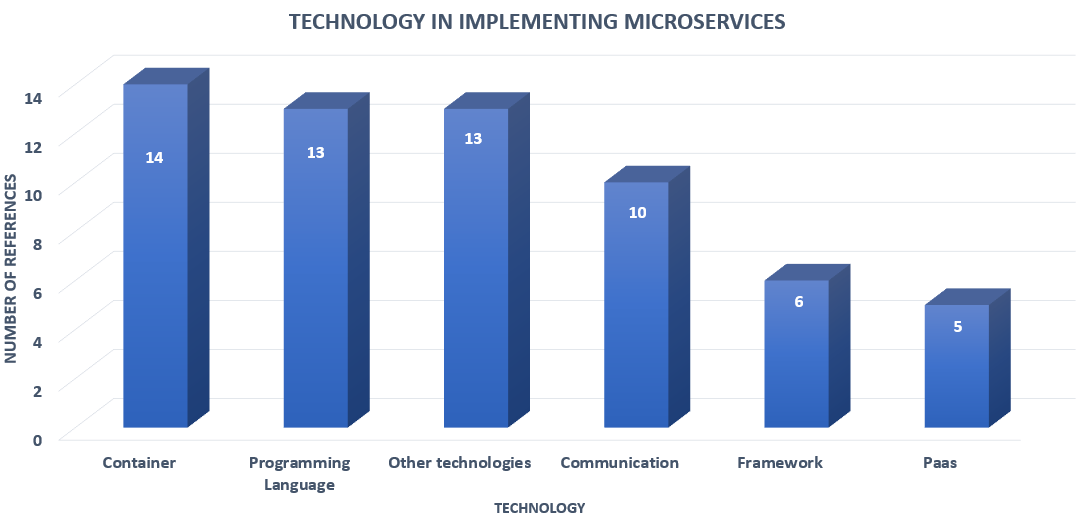
\includegraphics[width=0.5\linewidth]{images/commtechother.png}
	\caption{Technologies per group used for Implementing Microservices}
	\label{fig:tech-group}
\end{figure}	

In this section, we discuss RQ\#2, which is about the technologies used in the implementation of microservices according to our studied sources. Figure~\ref{fig:tech-group} shows the major groups of technologies that appeared in our studied references. We classified the technologies into \techgroupcount major groups.
Figure~\ref{fig:tech-distinct} shows the distinct technologies proposed to implement microservices. In total, we discovered \techcount different technologies in our data. 
The number of references of the groups showed in Figure~\ref{fig:tech-group} is the union of the references of the distinct technologies (Figure~\ref{fig:tech-distinct}) we classified in each group.  

\begin{figure*}[t]
	\centering
	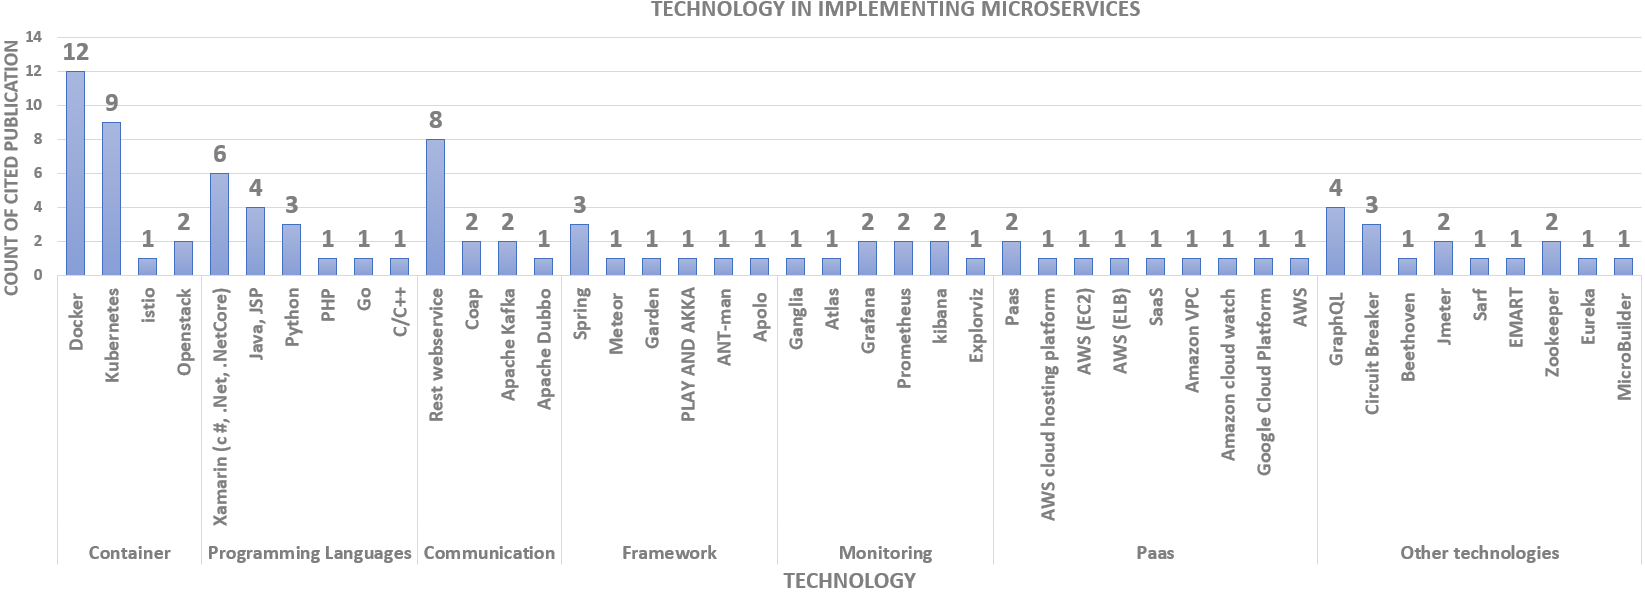
\includegraphics[width=\linewidth]{images/commontechupdated.png}
	\caption{Technologies in implementing microservices }
	\label{fig:tech-distinct}
\end{figure*}


\subsubsection{Containers}
Containers encapsulate discrete components of application logic provisioned only with the minimal resources needed to do their job. Containers and microservices enable developers to build and manage self-healing microservice-based applications more easily.
 
\par Docker: Docker is a platform for developing, shipping, and running applications. Developers can implement applications very fast by using docker~\cite{Sharaf2019, Kristiani2020, khan2020}. Moreover, it is simpler to create required services separately and manage them as microservices without affecting other services~\cite{leo2019, Hou2020, Kalske2017, Bahadori2018}. We can create a docker image for service and by running some docker commands, we can view our microservice application inside a docker container. Docker swarm applications can be deployed as services in a swarm cluster~\cite{Falatiuk2019, Venugopal2017, coulson2020}.
	
\par Kubernetes: Kubernetes is a container orchestration system that is well-suited to automate the management, scaling, and deploying of microservice applications~\cite{Zaytev2018, Kristiani2020, khan2020}. 
It is also possible to run kubernetes locally using MiniKube~\cite{leo2019, Kalske2017}.
Kubernetes ensures that the desired state (i.e., the state that we want the system to be in) and the actual state (i.e., the state that the system is actually in) are always in sync. Kubernetes continuously monitors the health of the cluster and ensures that the system is self-healing~\cite{Bahadori2018, Falatiuk2019, Venugopal2017}.

\par OpenShift: Red hat openshift is an open-source container application platform based on the kubernetes container orchestrator for enterprise application development and deployment~\cite{Johansson2019, Bahadori2018}.


\subsubsection{Programming Language}
When it comes to microservices development, a natural question is what language to choose. Developers have many options regarding programming languages to develop microservices. The programming languages mentioned in the citations are shown below.

\par Xamarin (C\#, .net, .netcore): asp.net, the web framework for .net, makes it easy to create the application programming interface to become microservices. Asp.net comes with built-in support for developing and deploying your microservices using docker containers~\cite{liu2018, chauvel2018, haugeland2020, Johansson2019, neves2019, Falatiuk2019}.

\par JAVA (Java, jsp): WSO2MicroservicesFramework for java has been used in implementing microservices~\cite{Sharaf2019, khan2020, KalskeM2017, Venugopal2017}.

\par Python: Python programming language uses flask application for building microservices~\cite{Ghebremicael2017, khan2020, Hou2020}.

\par PHP: PHP is also another programming language that can be used for implementing microservices~\cite{McElhiney2018}.

\par Go: Golang, also known as 'go' is popular for its concurrency and application programming interface support in terms of microservices architecture. It can be a good choice for microservices development. ~\cite{liu2018}.

\par C/C++: C++ is a programming language with imperative and object-oriented features that help developers write fast, portable programs. C++ is especially popular in areas where performance is crucial. Also, the compilation time and execution time of c++ is much faster than most other programming languages~\cite{Ghebremicael2017}. 


\subsubsection{Communication}

The goal of the microservice architecture is to create loosely coupled services, and communication plays a key role in achieving that. Therefore, services must interact using interprocess communication protocols such as http, amqp, or a binary protocol like transmission control protocol (TCP), depending on the nature of each service. Below we present the communication protocols used in the studied publications and grey literature.

\par REST API: REST API stands for 'representational state transfer' and It is a set of rules that developers follow when they create their application programming interface~\cite{Ndungu2019, Zhang2019}. One of the rules states that a user should be able to get a piece of data by using a specific URL~\cite{Koschel2017, Branko2018}. Microservices function as the building blocks of the application by performing various services, while restful application programming interface function as the communication that integrates the microservices into an application.\cite{liu2018, Zaytev2018, chauvel2018, Johansson2019}.

\par CoAP: CoAP and http are both based on the rest model and can be used as communication protocols to expose restful Web Services in a mobile device cloud. We will compare coap with http to better explain it. coap is a restful web transfer protocol optimized for communication between resource-constrained networks and nodes. CoAP uses the User datagram protocol (UDP) as its transport protocol, unlike http which operates on top of the reliable transmission control protocol and can be too complex for constrained environments. CoAP is not a blind compressed version of http, but a subset of rest common, with support of uniform resource identifier (URI) and http verbs, that gear towards machine-to-machine applications, hence it is an effective protocol for micro-services hosted on mobile devices~\cite{liu2018, khan2017}.

\par Apache Kafka: Apache kafka is an open-source distributed event streaming platform. Apache kafka is a powerful instrument for microservice architectures, which solves a variety of problems such as low-latency ingestion of large amounts of event data~\cite{wang2020, ebay}.

\par Apache Dubbo: Apache dubbo is a remote procedure call or remote procedure control-based service framework for programming. Dubbo is also a service governance framework, which provides service governance solutions such as service discovery and traffic scheduling for distributed microservices~\cite{Zhang2019}


\subsubsection{Framework}

Microservices can be implemented with a plethora of frameworks and using frameworks can help speed up the development of microservices. Below we present the frameworks used in implementing microservices in the analyzed references.

\par Spring framework: Spring is an open-source framework based on the java platform. Spring boot is part of the spring framework family to fastly create stand-alone applications. The distributed nature of microservices brings challenges. Spring helps us mitigate these. With several ready-to-run cloud patterns, spring cloud can help with service discovery, load-balancing, circuit-breaking, distributed tracing, and monitoring. It can even act as an application programming interface gateway ~\cite{KalskeM2017, selmadji2020, Santos2020}.

\par Meteor framework: Meteor is a framework meant to facilitate the whole web application development, encompassing the frontend, backend, as well as database. As such, it can be considered a full-stack web application framework. Meteor is written in javascript and is based on Node.js. The concept of having a proper microservices architecture using multiple meteor applications should be achieved reliably ~\cite{Tuuli2020}.


\par Apollo framework: Apollo is a great fit with microservice architectures and modern user interface frameworks like React. It serves as an abstraction layer that decouples services and applications so that each can be developed independently of the other, in any language and on any platform ~\cite{Kevin2015}.

\par Garden framework: Garden framework works like a spinnaker for implementing microservices~\cite{Ellen2018}.

\par ANT-man framework: an auto, native and transparent power management framework that can exploit fine-grained microservice variability for system efficiency\cite{Hou2020}.


\subsubsection{Monitoring}
Monitoring is a process of reporting, gathering and storing data. Some of the technologies/tools which are discussed before for monitoring microservices. 
\par Ganglia: Ganglia is one of the distributed monitoring tools for high-performance computing systems~\cite{Kristiani2020}.

\par Atlas: Atlas is a cloud monitoring tool which is newly introduced by netflix~\cite{Netflix}.

\par Explorviz: Explorviz is a monitoring and visualization approach, which uses dynamic analysis techniques to provide a live trace visualization of large software landscapes\cite{Lenga2019}.

\par Play AND Akka: The play framework is a web framework for the java virtual machine (JVM) that breaks away from the servlet specification. Play embraces a fully reactive programming model through the use of futures for asynchronous programming, work stealing for maximizing available threads, and akka for distribution of work. They are useful in building individual services, and leveraging both http and kafka for inter-service communication~\cite{khan2017}.

\par Grafana: Grafana is an open-source platform for data visualization, monitoring and analysis~\cite{KalskeM2017,Kalske2017}. 

\par Prometheus: Prometheus is an open-source monitoring system with a dimensional data model, flexible query language, efficient time series database and modern alerting approach~\cite{KalskeM2017, Kalske2017} 

\par Kibana: Kibana is a free and open user interface that lets us visualize your elasticsearch data and navigate the Elastic Stack~\cite{KalskeM2017, Kalske2017} 


\subsubsection{Platform as a Service (PaaS)}

Running microservices on a platform as a service fabric decreases solution fragility, reduces operational burden, and enhances developer productivity~\cite{rosa2018, Mikail2020}.

\par Amazon web services (AWS) cloud hosting platform: Among the primary benefits of a microservices architecture are the utilization and cost benefits associated with deploying and scaling components individually. While these benefits would still be present to some extent with on-premises infrastructure, the combination of small, independently scalable components coupled with on-demand, pay-per-use infrastructure is where real cost optimizations can be found~\cite{McElhiney2018}.

\par AWS auto-scaling group (EC2): Amazon elastic compute cloud is a part of amazon cloud-computing platform, amazon web services, that allows users to rent virtual computers on which to run their computer applications~\cite{McElhiney2018}.

\par Amazon AWS elastic load balancer: Elastic load balancing automatically distributes incoming application traffic across multiple targets~\cite{McElhiney2018}.

\par Software as a service (SaaS): Microservices are the resulting standalone services after breaking a software application down into separate components that perform their functions without being embedded in the application itself. Microservices are perfectly suited for saas, where each service is assumed to be part of a larger system~\cite{haugeland2020}.

\par Amazon VPC: Amazon virtual private cloud (Amazon VPC) is a service that lets us launch aws resources in a logically isolated virtual network that we define. Amazon~\cite{Amazon} uses amazon vpc to secure the traffic across cloud.

\par AWS Lamdba: AWS lamdba is a compute service that lets us run code without provisioning or managing servers. Lambda runs the code only when needed and scales automatically. AWS lambda is used to reduce infrastructure costs~\cite{villamizar2017}.

\subsubsection{Other Technologies}

\par GraphQL: Graph query language (GraphQL) is considered as an alternative for Representational state transfer application programming interface. It is most useful when it is able to combine different data sources into one and serve that up as one unified application programming interface. GraphQL hides the fact that we have a microservice architecture from the clients. From a backend perspective, we want to split everything into microservices, but from a frontend perspective, we would like all our data to come from a single application programming interface. Using graphgl is the best way that lets us do both~\cite{Ghebremicael2017, wang2020, overeem2018, gozneli2020}.

\par Circuit breaker: Hystrix, circuit breaker pattern allows us to build a fault-tolerant and resilient system that can survive gracefully when key services are either unavailable or have high latency \cite{Kalske2017}, \cite{Rodrigue2016}, \cite{Uber}. 

\par Beethoven: Beethoven is a platform composed of a reference architecture and a domain-specific language for expressing microservice communication flows~\cite{Monteiro2020}.

\par Apache JMeter: Apache jmeter is an apache project that can be used as a load testing tool for analyzing and measuring the performance of a variety of services. It is also used for performance-test in the microservice applications ~\cite{Hou2019}~\cite{Johansson2019}.

\par SArF : SArF is an sofware clustering algorithm and it has two characteristics. First, sarf eliminates the need of the omnipresent-module-removing step which requires human interactions. Second, the objective of sarf is to gather relevant software features or functionalities into a cluster. Thus, it is used to find the candidates for microservice from the source code ~\cite{Kamimura2018}.

\par EMART: Enhanced microservice adaptive reliability testing (EMART) is a tool for testing the applications~\cite{Russo2020}

\par Apache Zookeeper: Apache zookeeper is an open-source server for highly reliable distributed coordination of cloud applications. However, this architecture makes it hard to scale out to huge numbers of clients. ZooKeeper node called an 'observer' which helps address this problem and further improves zooKeeper's scalability~\cite{Kalske2017, KalskeM2017}.


\par Eureka Server: Eureka server is an application that holds the information about all client-service applications. Every micro service will register into the eureka server and Eureka server knows all the client applications running on each port and internet protocol address~\cite{Uber}.


\par MicroBuilder: MicroBuilder is the tool used for the specification of software architecture that follows representational state transfer microservice design principles~\cite{Branko2018} 


